
%\documentclass[12pt]{amsart}
%\usepackage{geometry} % see geometry.pdf on how to lay out the page. There's lots.
%\usepackage{datetime}
%\usepackage{setspace}
%\doublespacing
%\geometry{a4paper} % or letter or a5paper or ... etc
%% \geometry{landscape} % rotated page geometry
%
%% See the ``Article customise'' template for come common customisations
%
%\title{Wind chapter}
%\author{Percy Link}
%\date{\currenttime \ \today} % delete this line to display the current date
%
%%%% BEGIN DOCUMENT
%\begin{document}
%
%\maketitle

\section{Methods}

The sensitivity of Solano wind forecasts to soil moisture is tested using numerical experiments with a regional atmospheric model, the Weather Research and Forecasting (WRF) model.  The WRF model, described in Section \ref{sec:BL_WRFdesc} and in detail in \cite{skamarock2008}, is a three-dimensional, non-hydrostatic regional atmospheric model with terrain-following vertical coordinates. WRF has been used extensively in wind energy forecasting [\cite{marjanovic2014}, \cite{wharton2011review}, \cite{carvalho2012sensitivity}, \cite{deppe2013wrf}, \cite{foley2012current}].

\subsection{Model setup}

We run WRF with two nested domains centered on the Solano wind farm (Figure \ref{fig:windSol_domainmap}); the domains are described in Table \ref{table:windSol_domains}.  As in Chapter \ref{c.BL}, the outer grid forces the lateral boundaries of the inner grid, and the inner grid feeds back to the outer grid across the region where the two domains overlap [\cite{skamarock2008}].  The outer and inner domain are Arakawa-C grids with horizontal resolution of 8.1 km and 2.7 km, respectively; preliminary tests with a third finer grid (0.9 km) showed little change in the forecasted winds, echoing the results of \cite{marjanovic2014}, who found little accuracy improvement with horizontal resolution below 2.7 km in their simple terrain case.  The domain has 45 vertical levels, with a minimum spacing of $\sim$30 m near the surface and increasing with height, interpolated quadratically by the log of pressure (the default WRF setting); turbine-level (60-100 m) wind forecasts are not very sensitive to vertical resolution beyond about 40 levels with this vertical interpolation scheme in WRF [\cite{marjanovic2014}, and references therein].

\begin{figure}[here]
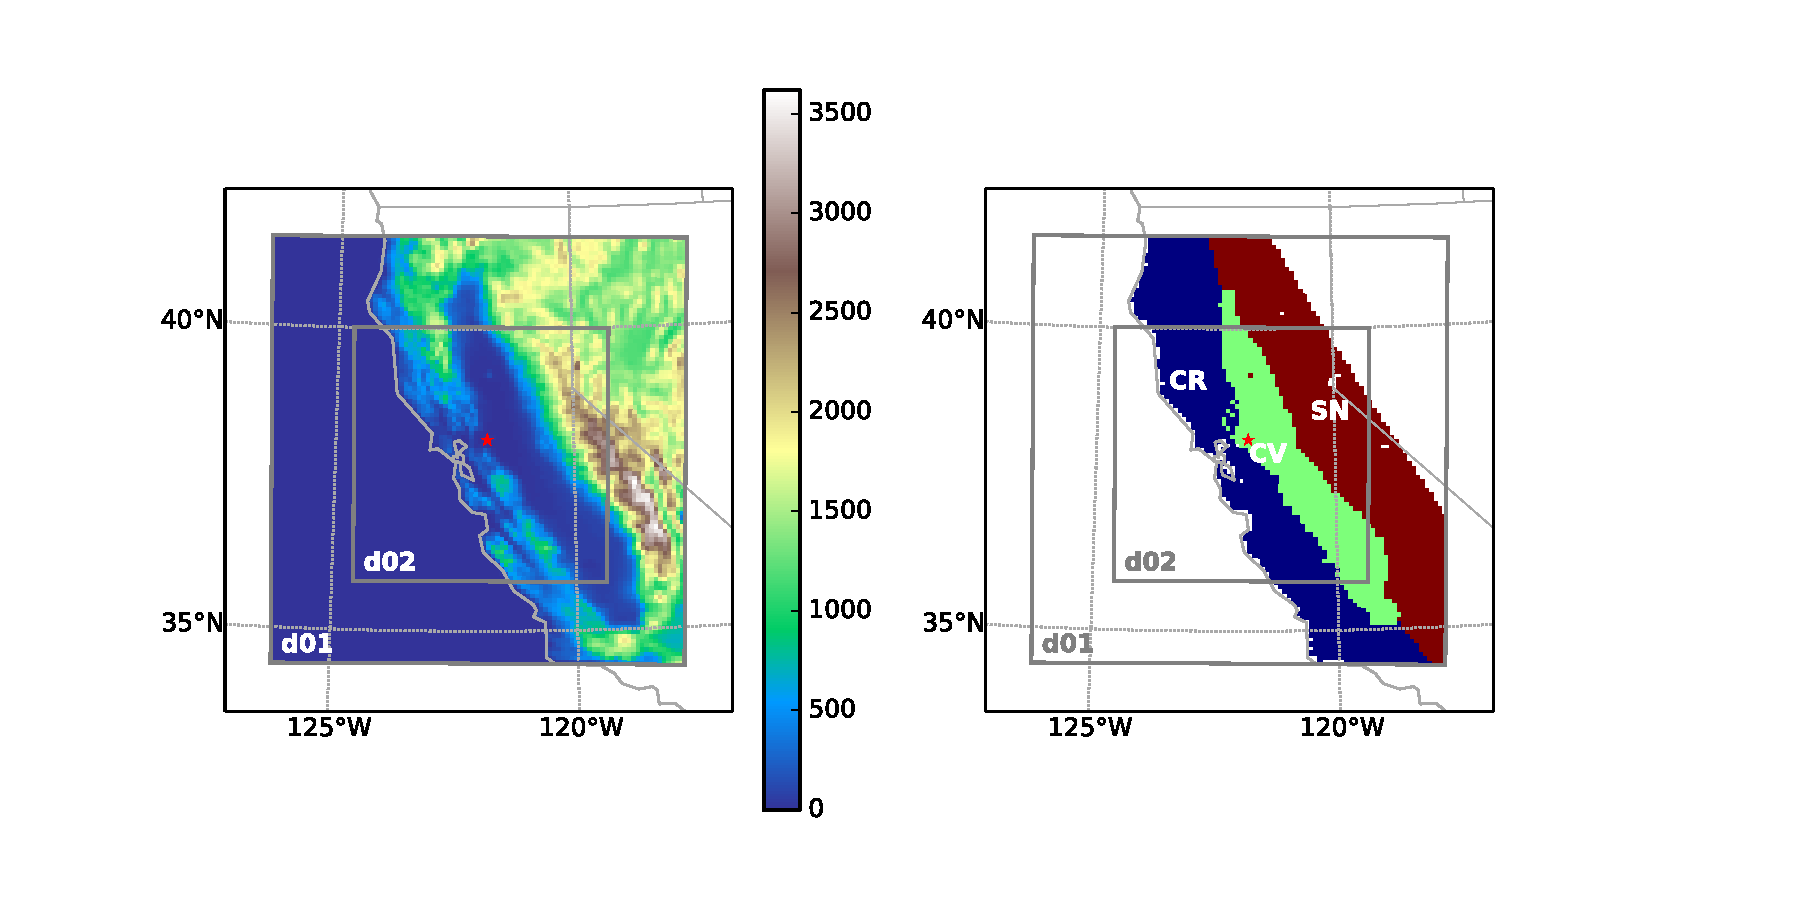
\includegraphics[width=1\textwidth]{ch3-wind/img/domain_map_cropped.pdf}
\caption{WRF model domains, showing (a) topographic height in m, and (b) regions used for soil moisture experiments in this study: the Coast Range (CR, blue), Central Valley (CV, green), and Sierra Nevada (SN, red). d01 refers to the outer model domain, and d02 refers to the inner domain.  The red star symbol shows the location of the Solano Wind Project.}
\label{fig:windSol_domainmap}
\end{figure}

\begin{table}
\begin{tabular}{ l c c c c c c c }
\hline
Domain & $\Delta x$ (km) & $\Delta y$ (km) & $nx$ & $ny$ & $nz$ & $\Delta t$ (s) & USGS data res \\ \hline
d01 & 8.1 & 8.1 & 96 & 99 & 45 & 45 & 2 min\\
d02 & 2.7 & 2.7 & 175 & 175 & 45 & 15 & 2 min\\
\hline
\end{tabular}
\caption{Model domains. d01 refers to the outer domain, and d02 refers to the inner domain.}
\label{table:windSol_domains}
\end{table}

In WRF, the atmospheric model is coupled to the Noah land surface model with 24-category USGS land use and 16-category soil classifications [\cite{skamarock2008}].  The observed distributions of land use and soil types are used [\cite{eidenshink19941}; \cite{miller1998conterminous}], as are the default vegetation water-use parameters for each land use type [\cite{skamarock2008}], in order to simulate as closely as possible the real present day sensitivity of Solano winds to soil moisture.  Uncertainties associated with errors in the model representation of water movement in the subsurface and plant water use are addressed in the Discussion. 

As in Chapter \ref{c.BL}, the ACM2 PBL scheme is used, following the recommendations of \cite{marjanovic2014} for a locally forced simple terrain case in California; this PBL scheme includes both local (small-scale turbulent) and nonlocal (large convective plume) vertical transport, and can thus simulate both stable and unstable conditions [\cite{pleim2007combined}] A LITTLE MORE DETAIL ABOUT THE PHYSICS.  The model is forced at the lateral boundaries with NCEP Eta 212 grid (40 km) operational analysis [\cite{ncep}].  Other parameterization schemes and settings are as in Table \ref{table:BL_paramschemes}.  Model variables are output every 30 minutes.

All experiments are run for the period 2009-06-26 00:00 UTC to 2009-07-11 00:00 UTC, and the first 32 hours are discarded as model spin-up.  This period was chosen for several reasons: (1) it contains a range of synoptic conditions (weak background wind June 27-July 5, and strong background wind July 6-11; Figure \textbf{XX}), (2) turbine-level wind speeds in this region are highest in the spring and summer [\cite{zhong2004diurnal}; \cite{mansbach2010synoptic}], and (3) the sensitivity to soil moisture is expected to be strongest in the warm season when radiation incident to the land surface is greatest, because changes in the relative partitioning between evapotranspiration and sensible heat flux have the largest absolute magnitude then.

\subsection{Soil moisture experiments}

We conduct three sets of model experiments, listed in Table \ref{table:windSol_runlist}.  In the first set of experiments, we test the sensitivity of Solano winds to soil moisture in different large-scale regions of California.  In cases dryCR, dryCV, and drySN, the background volumetric soil moisture (model variable SMOIS, m$^3$ water/m$^3$ total volume) is set to a moderately wet value of 0.25, and the soil moisture of the test region (respectively, the Coast Range, Central Valley, and Sierra Nevada, shown in Figure \ref{fig:windSol_domainmap}b) is set to a dry value of 0.1.  These test cases are compared with a control case where all land has the moderately wet soil moisture value of 0.25.  In cases wetCR, wetCV, and wetSN, the background soil moisture is set to the dry value of 0.1, and the soil moisture of the test region is set to the moderately wet value of 0.25.  These test cases are compared with a control case where all land has the dry soil moisture value of 0.1.  For reference, climatological soil moisture, using North American Regional Reanalysis (NARR) monthly averaged soil moisture from 1979-2014, is shown in Figure \ref{fig:windSol_NARR_smois}.  A soil moisture value of 0.1 m$^3$/m$^3$  represents an abnormally dry July state for the Coast Range and Sierra Nevada and a moderately dry July state for the Central Valley.  A soil moisture value of 0.25 m$^3$/m$^3$  represents an abnormally wet July state for the Central Valley and southern Coast Range, a moderately wet July state for the northern Coast Range, and a typical July state for the Sierra Nevada.  The NARR soil moisture reanalysis is presented with the caveats that the soil properties (\textit{e.g.} field capacity) may vary between the soil dataset used in NARR and the one used in this study, and that there are known errors in NWP-derived soil moistures [\cite{marshall2003impact}; \cite{godfrey2008soil}].

\begin{figure}[here]
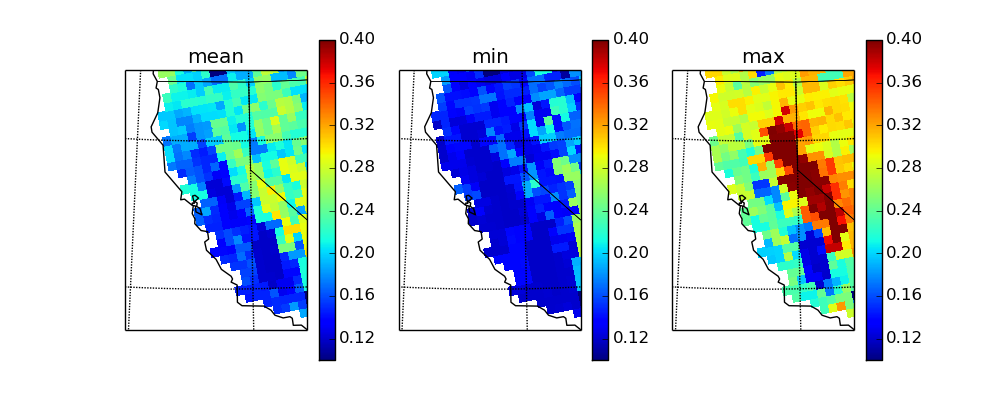
\includegraphics[width=1\textwidth]{ch3-wind/img/NARR_smois_maps_3.png}
\caption{July monthly-mean volumetric soil moisture (m$^3$/m$^3$) from the North American Regional Reanalysis (NARR) dataset, 1979-2014, depth-weighted average over the top 100 cm.  Left, center, and right panels show, respectively, the average, minimum, and maximum July soil moisture for each grid point for 1979-2014.}
\label{fig:windSol_NARR_smois}
\end{figure}

The next set of experiments tests how the Solano wind response scales with soil moisture in the Central Valley, with a normal-to-wet background in the Coast Range and Sierra Nevada.  In cases CVXX (where XX is a numeric value), the Coast Range and Sierra Nevada regions' soil moisture is set to 0.2, and the Central Valley soil moisture is set to the value specified by XX.  These test cases are compared with a control case where all land has soil moisture of 0.2.
%In cases CVXXdry, the Coast Range and Sierra Nevada regions' soil moisture is set to 0.1, and the Central Valley soil moisture again is specified by XX.

In all cases, the soil moisture is set to the prescribed values at the model start time (2009-06-26 00:00 UTC) and is reset to the prescribed value each day at 08:00 UTC (midnight Pacific Standard Time); the soil moisture evolves according to the land surface model each day between resets.  The change in soil moisture between resets is small (up to 0.02 m$^3$/m$^3$ in the regional average when soils are wet and much less when soils are dry.  Additionally, the synoptic forcing, measured by wind speed at 500 hPa, varies little between the model runs (Figure XX), and synoptic winds are weak on June 27 to July 5 and strong on July 6 to 11.  In all three regions, land surface sensible heat flux is approximately 200 W/m$^2$ greater at midday with wet soil moisture (0.25) than dry soil moisture (0.1).  \textbf{Need to make figure showing these.}

%\begin{figure}[here]
%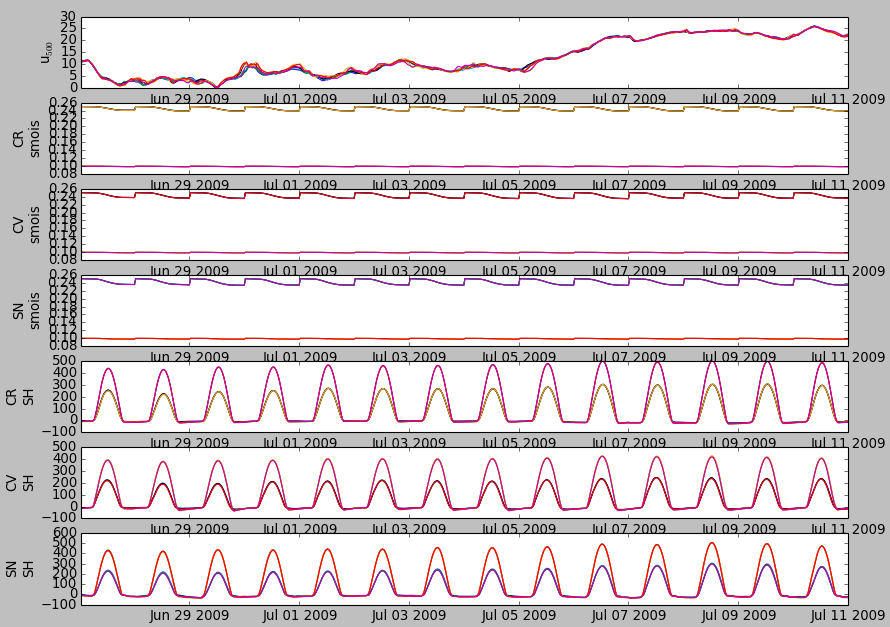
\includegraphics[width=1\textwidth]{ch3-wind/img/forcings_combo_good.png}
%\caption{Model forcing for all of the regional perturbation cases.  \textbf{I NEED ADVICE ON HOW TO DISPLAY THIS INFORMATION MORE CLEARLY AND/OR CONCISELY. Obviously, I need a legend for which color means which run.}  Top panel: wind speed over Solano at 500 hPa.  Panels 2-4: average soil moisture in the top soil layer for the CR region (panel 2), the CV region (panel 3), and the SN region (panel 4).  Panels 5-7: average surface sensible heat flux for the CR region (panel 5), the CV region (panel 6), and the SN region (panel 7).}
%\label{fig:windSol_forcings}
%\end{figure}

\begin{table}
\begin{tabular}{p{2.5cm} l p{3cm} p{3cm} p{3.5cm}}
\hline
Experiment & Run name & Background SMOIS (kg/kg) & Perturbed SMOIS region & Perturbed SMOIS value (kg/kg) \\
\hline
1 & CA-0.1 & 0.1 & none & n/a \\
1 & wetCR & 0.1 & Coast Range & 0.25 \\
1 & wetCV & 0.1 & Central Valley & 0.25 \\
1 & wetSN & 0.1 & Sierra Nevada & 0.25 \\
2 & CA-0.25 & 0.25 & none & n/a \\
2 & dryCR & 0.25 & Coast Range & 0.1 \\
2 & dryCV & 0.25 & Central Valley & 0.1 \\
2 & drySN & 0.25 & Sierra Nevada & 0.1 \\
3 & CA-0.2 & 0.2 & none & n/a \\
3 & CV0.05 & 0.2 & Central Valley & 0.05 \\
3 & CV0.1 & 0.2 & Central Valley & 0.1 \\
3 & CV0.15 & 0.2 & Central Valley & 0.15 \\
3 & CV0.25 & 0.2 & Central Valley & 0.25 \\
3 & CV0.3 & 0.2 & Central Valley & 0.3 \\
3 & CV0.35 & 0.2 & Central Valley & 0.35 \\
%CV0.05dry & 0.1 & Central Valley & 0.05 \\
%CV0.15dry & 0.1 & Central Valley & 0.15 \\
%CV0.2dry & 0.1 & Central Valley & 0.2 \\
%CV0.25dry & 0.1 & Central Valley & 0.25 \\
%CV0.3dry & 0.1 & Central Valley & 0.3 \\
%CV0.35dry & 0.1 & Central Valley & 0.35 \\
\hline
\end{tabular}
\caption{Model experiments, using regions shown in Figure \ref{fig:windSol_domainmap}(b): (1) Dry background, wet perturbation region; (2) Wet background, dry perturbation region; (3) Sensitivity to Central Valley soil moisture.}
\label{table:windSol_runlist}
\end{table}

\subsection{Analysis of model output}
\label{subsec:methods_model_output}

The winds at turbine hub height at the Solano Wind Project are approximated using 60 m above ground level (AGL) winds at the WRF model grid point closest to 38.166N, 121.817W.  The rolling hills at the Solano Wind Project have a terrain height of 40-60 m; thus, the wind at hypothetical 60 m AGL wind turbine hubs at the Solano Wind Project is approximated using wind from 110 m above sea level (ASL).  All times are expressed in local time (Pacific Standard Time).

Two types of anomalies are analyzed.  The first is the anomaly at each grid point ($i$, $j$), altitude ($z$), and time ($t$), from the horizontal average pressure at that altitude and time ($\widehat{p_{z, t}}$):
\begin{equation}
\delta p_{i, j, z, t} = p_{i, j, z, t} - \widehat{p_{z, t}}.
\end{equation}
The second anomaly is the difference between a test case and its corresponding control case:
\begin{equation}
\Delta x = x_{test} - x_{control}
\end{equation}
for an arbitrary variable x.


%\end{document}